\documentclass[11pt]{article}
\usepackage[margin=1in]{geometry}
\usepackage[T1]{fontenc}
\usepackage[utf8]{inputenc}
\usepackage{lmodern}
\usepackage{amsmath}
\usepackage{booktabs}
\usepackage{graphicx}
\usepackage{caption}
\usepackage{enumitem}
\PassOptionsToPackage{hyphens}{url}
\usepackage[hidelinks]{hyperref}
\usepackage{microtype}

\title{Self-Simulation in a Learned World Model:\\ What an Agent Can Know About Its Own Discovery Rates\\ from Experience It Earned Itself}
\author{Maureese Williams}
\date{October 10, 2026}

\begin{document}
\maketitle

\begin{abstract}
An agent that has lived through 1,280 worlds, keeping only the atoms behind the picks it could tell were reliable, can build a model of those worlds and of itself that predicts how often it will find each atom to within 0.02 mean absolute error of a second independent run of the true generator. Each world is 14 atoms drawn from 3 of 7 families and admits about 160 rules, and the agent earns atoms by solving tasks under a fixed scan budget with no outcome feedback. From the earned sets alone, a joint expectation-maximization fit recovers which atoms travel together (adjusted Rand 0.90 and 0.93 against the families on two seeds, 0.62 on the third), how often each family combination occurs, and which atoms it only ever meets through its own mistakes. The agent then imagines worlds from this model and lives them with its own policy and tie-break. Within every family whose atoms differ measurably in discoverability, the imagined discovery rates match the benchmark as well as the benchmark's two halves match each other. Pooled over atoms the correlation is 0.17 to 0.39 against a ceiling of 0.78, and this gap is entirely the family mix. Imagined worlds contain the largest family, mod, 64\% of the time against 35\% in reality, because the smallest family, rotmod, never receives a group of its own and its worlds are filed under mod. The cause is identified and not yet fixed. Each atom's import rate, the chance of earning it by a wrong pick, is a free parameter, so an atom filed under the wrong group costs the likelihood nothing. Two measurement errors were found and corrected along the way. The benchmark had been drawn from a population of worlds the agent never lived in, and two samplers redrew the family combination on any rejection and so hid the mix error.
\end{abstract}

\section{Introduction}

The programme behind this work asks whether an agent can grow by earning every level of its own machinery instead of being handed it. The machinery is arranged in four levels. L0 is the solver, one rule that orders the hypothesis catalog, scans it, submits a hypothesis and keeps the atoms of what it submitted, and its resource is scans per task. L1 is the world model, a grouping of atoms and a posterior over which groups the current world uses, and its resource is worlds lived. L2 is the representation learner that turns earned world sets into an L1, and L3 is a selector that chooses an L2 from the early statistics of a new environment. Every level is meant to be earned, hedged, and held to a label-free internal evaluator.

Four claims were confirmed before this work, each predeclared and audited. Experience of a world's mechanisms raises solving within that world (G1). A prior learned across worlds transfers to family combinations never trained (G2). A family-level world model moves the tight-budget wall that no policy over the agent's own evidence could move (C-family). A grouping learned from world atom sets without labels improves acquisition with worlds seen, past the point where the pairwise prior saturates (C-growth).

C-growth left an accounting gap. Its groups were learned from true atom sets that were handed to the learner, so the representation level was the one level where experience was not charged. The C-earned confirmation of 2026-10-05 charged it. Groups were learned from atoms the agent itself had earned under a scan budget, and the growth and structure gates passed in both replications while the safety gate failed in both, with losses of up to 350 of 12,800 tasks at budgets 256 and 512. The earned grouping covered about half the atoms and recovered a quarter of the handed gain.

This paper is the step between that failure and the next deployment. Before an earned L1 is deployed again, I ask whether it is a faithful model of the worlds the agent lived in and of the agent itself, measured by what it makes the agent predict about its own discovery. A representation that is wrong about how often the agent will find each atom cannot set its own trust, because trust is exactly a prediction of that kind. The deployment question, whether the model raises acquisition, is deferred until the prediction holds.

\section{The environment}

A mechanism is one of 166,596 behaviourally distinct character predicates written in the host language's own expression grammar. Each predicate is built from one or two atoms, and there are 313 atoms in 9 families named after the arithmetic operation they apply. The families differ widely in size. The mod family has 135 atoms, divmod 50, popcount 39, xormod 30, bit 16, threshold 15, parity 14, rotmod 8 and gcd 6. The family is a fact about the atom's syntax, not its behaviour. Clustering atoms by what they compute recovers the family labelling at adjusted Rand 0.14, so nothing computable on an atom alone can see its family.

A world is 14 atoms drawn uniformly from the pooled atoms of 3 families, kept only if all 3 families appear and the 14 atoms generate at least 130 catalog predicates. A world admits about 160 predicates on average. The generator keeps the family triple and redraws the atoms on a rejection, up to 40 times, so the filter changes which atoms a triple yields and not how often each triple occurs. Popcount and xormod are held out. The agent never lives in a world that uses them, but it can earn their atoms through its own wrong picks. Of the 35 triples over the remaining 7 families, 31 are viable, and 20\% of those are reserved as untrained combinations for later transfer tests, so an agent trains on 26 triples at seeds 643101 and 644101 and 24 at 645101.

The agent lives a world as a stream of 100 tasks. A task shows a few visible positive and negative examples of one of the world's predicates and holds further examples hidden. The agent scans the first 4,096 entries of the catalog in its own order, and among the entries consistent with the visible examples it submits the smallest. Whether the submission satisfies the hidden examples is scored but never shown. The agent keeps the atoms of whatever it submitted. This is the earned loop, and it closes without feedback: an agent that keeps its submitted atoms raises its own solve rate four to ten times over a lifetime at every budget from 128 to 4,096 scans.

The agent can tell its reliable picks from the rest without being told. The signal is the number of consistent hypotheses it found inside the budget before submitting. When it found exactly one, the pick is correct 90\% of the time. When it found more than 16, the pick is correct 26\% of the time. This work uses the picks with one consistent hypothesis, called confident picks, as the evidence the world model is fitted on, and reports the fit on all picks beside it.

Three development seeds, 643101, 644101 and 645101, each supply 1,600 training worlds. The first 1,280 fit the model and the remaining 320 score held-out likelihood. Every lifetime is replayed with the agent's own tie-break, because its scan order among equally scored hypotheses is part of what it will and will not find.

\section{Why earned groups failed: discovery bias}

The representation learner that passed C-growth clusters atoms by the pointwise mutual information of their co-occurrence across worlds, with the group count chosen by held-out likelihood. Fed the true atom sets of 1,600 worlds it recovers the families at adjusted Rand 0.87 to 0.89, merging only rotmod into mod. Fed the atoms the agent earned in the same worlds it recovers them at 0.17 to 0.55, and more worlds make it worse.

The cause is that earning is not a uniform sample of a world. Blind earning at 4,096 scans recovers 74\% to 84\% of a world's mod atoms and 23\% to 31\% of its rotmod and gcd atoms, because the catalog order reaches some families' predicates long before others'. Co-occurrence counted over earned sets therefore measures discoverability as much as membership, and a learner that reads more such worlds learns the bias with more confidence. Denoising by pick recurrence did not remove it. A generational bootstrap, where each generation earns with the previous generation's groups, raised solving from 27 to 36 tasks per world but left the grouping at adjusted Rand 0.36 to 0.53. Leaving atoms earned in fewer than 50 worlds ungrouped recovered enough structure to pass the growth and structure gates, and the safety gate then failed where the posterior committed to a wrong group on few observations.

Two conclusions follow. First, a world model built from earned experience must separate two quantities that earned sets confound, how often an atom is in a world and how often the agent finds it when it is. Second, the agent cannot be told the second quantity. It has to measure it on itself.

\section{The world and self model}

The model tells one generative story for a world and for the agent's experience of it. A world draws a set of three groups from a learned distribution $\pi$ over group sets, then draws its 14 atoms from the union of those groups in proportion to a per-atom prevalence weight. The agent then earns each atom that is in the world with probability $r$, its discovery rate, and each atom that is not with probability $f$, its import rate, the chance of earning it through a wrong pick. Atoms the agent has never earned are outside the model. The parameters are a group label per atom, $\pi$, $r$ and $f$ per atom, and the prevalence weights.

The fit is expectation-maximization over the binary worlds-by-atoms matrix of earned sets. The E step computes the posterior over group sets for each world. The M step updates $\pi$ from the posterior counts with light smoothing, updates $f$ from the earns the posterior attributes to non-members, updates $r$ from the earns it attributes to members, and reassigns each atom to the group under which its earned column has the highest expected log likelihood, holding the world posteriors fixed. An atom may also be assigned to no group, when its column is better explained by a constant import rate than by membership in any group, which is how atoms met only through wrong picks are recognised. The spectral start is followed by restarts that move a share of atoms to random groups, and the best training likelihood is kept. The group count is chosen by held-out likelihood on the last 320 worlds.

Two facts about identifiability shaped the design. From earned sets alone, $r$ and prevalence are not separable, because an atom earned in one world in ten may be a common atom the agent rarely finds or a rare atom it always finds. The first fit confirmed this. On sets of every pick the self model's discovery rates matched the truth at Pearson 0.67 to 0.71 with mean absolute error 0.15, and on sets restricted to picks repeated three times the correlation fell to 0.08. The world model was less affected. Its membership probabilities for held-out worlds reached area under the curve 0.86 against 0.79 for the earned set alone and 0.79 to 0.84 for the pairwise prior.

The second fact gives the model a way out. If $r$ is fixed from outside, prevalence becomes identifiable and is fitted. Section 5 describes how the agent can measure $r$ on itself. In the fits reported here $r$ is the expectation-maximization estimate and the weights stay at one, because feeding the measured $r$ back did not help while the world model was wrong. A further binding closes the loop in the other direction. An atom the self model says the agent would almost never find if it were in a world, $r$ below 0.10, is treated as being in no world, because the agent's experience of it can only have come through imports. Real atoms have $r$ between 0.37 and 1.0 and import-only atoms between 0.01 and 0.09, so the rule separates them cleanly, and it correctly excludes every popcount and xormod atom. It also excludes a few real atoms that are rarely found, about 20 of mod and 5 of divmod, which is a cost noted in Section 8.

\section{Self-simulation}

The agent measures its own discovery rates by living worlds it imagines. It draws 800 worlds from the fitted model, a group set from $\pi$ and then 14 atoms from the union of those groups in proportion to prevalence, and keeps a world only if its atoms generate at least 130 catalog predicates. On a rejection it redraws the atoms and keeps the group set, as the true generator does. The predicates of each imagined world become a stream of 100 tasks built by the same task generator, and the agent lives them with the same policy, the same 4,096-scan budget and its own tie-break. For every atom it counts the worlds in which the atom was present and the worlds in which it earned the atom, and the ratio is its imagined discovery rate. Nothing in this loop reads a true world, a family or a label. Ground truth enters only when the result is scored.

The simulation itself is faithful. Given the true world distribution instead of the fitted model, imagined discovery rates match the agent's real rates at Pearson 0.91 with mean absolute error 0.07, against 0.89 for two halves of the truth compared with each other. Inside the first fitted world model the same procedure reached 0.14 to 0.40. The world model, not the simulation, was the bottleneck, and the rest of this paper is about closing that gap.

A feedback loop was tried first and set aside. Fixing $r$ at the self-simulated value and refitting with prevalence weights made the discovery rates worse over two rounds on every seed, from Pearson 0.71 to 0.14 at 643101, 0.67 to 0.33 at 644101 and 0.54 to 0.33 at 645101, because worlds imagined from a wrong model teach the agent wrong things about itself. The completeness results below therefore fit $r$ by expectation-maximization with unit prevalence and use self-simulation only as the measurement. The loop stays available for a model that is complete.

One further finding about what counts as the agent's real rate. The confirmation protocol removes the mechanisms of the evaluation worlds from every training stream, and this removal shifts per-atom discovery rates. An oracle run on the training worlds without the removal matched the real training rates at Pearson 0.50 only. Training-world statistics are therefore not test conditions, and the benchmark of Section 6 runs the agent without any removal.

\section{Measuring completeness}

The benchmark is the same agent, with the same tie-break, living 1,600 worlds from the true generator with no mechanism removal, and counting for every atom the worlds in which it was present and the worlds in which it was earned. The 1,600 worlds are split into two independent halves of 800, and the agreement between the halves on the same atoms is the ceiling any model can be held to. Pooled over the 242 to 244 atoms present at least ten times in each half, the ceiling is Pearson 0.87 to 0.90 and mean absolute error 0.06 to 0.07.

A single pooled number misleads here, and the first pass of this work was misled by it. Within most families atoms barely differ in how often they are found. Within mod, the 135-atom family that makes up more than half of every pooled correlation, the two halves of the benchmark agree at Pearson 0.21 to 0.27, and within gcd and rotmod, with 6 and 8 atoms, the split-half agreement swings between seeds. Within bit, parity and threshold the halves agree at 0.87 to 0.99. A pooled Pearson is therefore mostly within-mod noise, and a model can be far from the ceiling on it while being right about every atom. Fidelity is reported per family, as the Pearson correlation between imagined and benchmark rates over the family's atoms, against the per-family split-half ceiling computed on exactly the same atoms. The mean absolute error per atom is reported beside it, because it does not share this weakness.

The benchmark must also be drawn from the population the agent lived in. The first benchmark drew its worlds from all 31 viable family triples, while the agent trains on 26, 26 or 24 of them, the rest being reserved as untrained combinations. At seed 644101 four of the six reserved triples contain mod, so mod appeared in 47\% of the first benchmark's worlds and in 35\% of the agent's training worlds. A world model true to the agent's experience would be scored as wrong by that benchmark on the very quantity it had learned. The final benchmark draws from each seed's training triple pool. Whether the model extends to untrained combinations is a question about generalization and is not asked here.

The family mix itself is reported directly, as atoms of each family per world in imagined worlds against the benchmark, because a model can be at the ceiling within every family and still imagine the wrong worlds.

\section{Results}

Fitted on confident picks, the world model recovers the families at adjusted Rand 0.93, 0.90 and 0.62 on seeds 643101, 644101 and 645101, with 6, 7 and 7 groups chosen by held-out likelihood and 224 to 232 of the 313 atoms grouped. Fitted on every pick it reaches 0.45, 0.67 and 0.65. Confident picks buy the structure. The third seed's 0.62 is a poor local optimum that four random restarts did not escape, and its within-family fidelity is unaffected by it.

\begin{figure}[t]
\centering
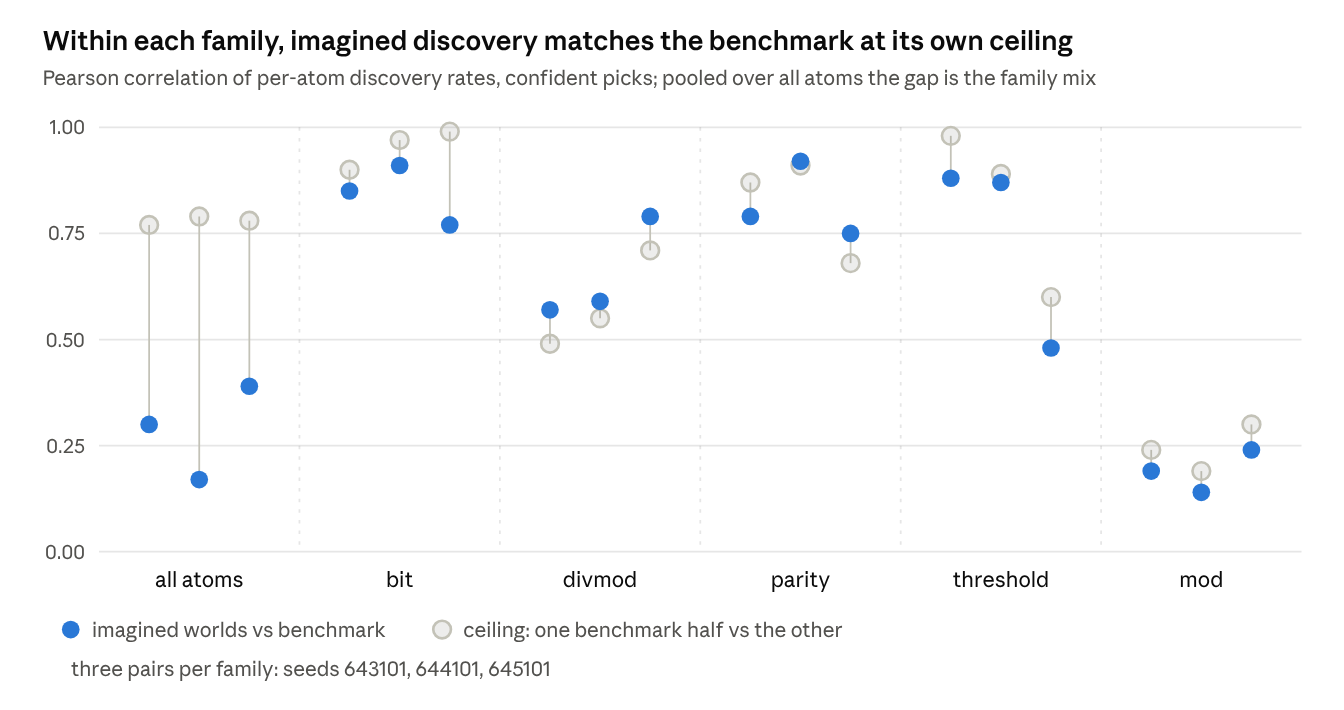
\includegraphics[width=\linewidth]{fig-fidelity.png}
\caption{Fidelity against ceiling, per family and pooled. Each filled dot is the Pearson correlation between imagined and benchmark discovery rates over a family's atoms at one seed, and the open dot above or below it is the correlation between the two benchmark halves on the same atoms. Three pairs per family are seeds 643101, 644101 and 645101. The first group pools all atoms.}
\label{fig:fidelity}
\end{figure}

Table~\ref{tab:fidelity} and Figure~\ref{fig:fidelity} give the per-family comparison. Within every family whose atoms differ measurably in discoverability, the imagined discovery rates match the benchmark as closely as its two halves match each other, on the same atoms, on all three seeds. Where the imagined correlation falls short of the ceiling, as for bit at 645101 (0.77 against 0.99) and threshold at the same seed (0.48 against 0.60), the ceiling itself is read from 14 to 16 atoms. For gcd and rotmod the comparison is possible only at 644101, where it gives 0.40 against 0.42 and 0.53 against 0.57. Per atom, the mean absolute error between imagined and benchmark rates is 0.080, 0.092 and 0.072 against a ceiling of 0.074, 0.068 and 0.063. Self-simulation inside the fitted model predicts how often the agent will find each atom about as well as a second run of the true generator does.

\begin{table}[t]
\centering
\caption{Discovery fidelity per family, confident picks. Fidelity is the Pearson correlation between imagined and benchmark discovery rates over the family's atoms; the ceiling is the same correlation between the two benchmark halves on the same atoms. Values for seeds 643101 / 644101 / 645101.}
\label{tab:fidelity}
\begin{tabular}{lccc}
\toprule
Family & Fidelity & Ceiling & Atoms \\
\midrule
bit & .85 / .91 / .77 & .90 / .97 / .99 & 14--16 \\
divmod & .57 / .59 / .79 & .49 / .55 / .71 & 46 \\
parity & .79 / .92 / .75 & .87 / .91 / .68 & 14 \\
threshold & .88 / .87 / .48 & .98 / .89 / .60 & 14--15 \\
mod & .19 / .14 / .24 & .24 / .19 / .30 & 125--132 \\
gcd (644101 only) & .40 & .42 & 6 \\
rotmod (644101 only) & .53 & .57 & 7 \\
\midrule
all atoms & .30 / .17 / .39 & .77 / .79 / .78 & 224--230 \\
mean absolute error per atom & .080 / .092 / .072 & .074 / .068 / .063 & \\
\bottomrule
\end{tabular}
\end{table}

Pooled over all atoms the correlation is 0.30, 0.17 and 0.39 against a ceiling of 0.78. The first group of Figure~\ref{fig:fidelity} shows the whole of this gap, and it is not in the atoms. It is in which worlds the model imagines.

\begin{figure}[t]
\centering
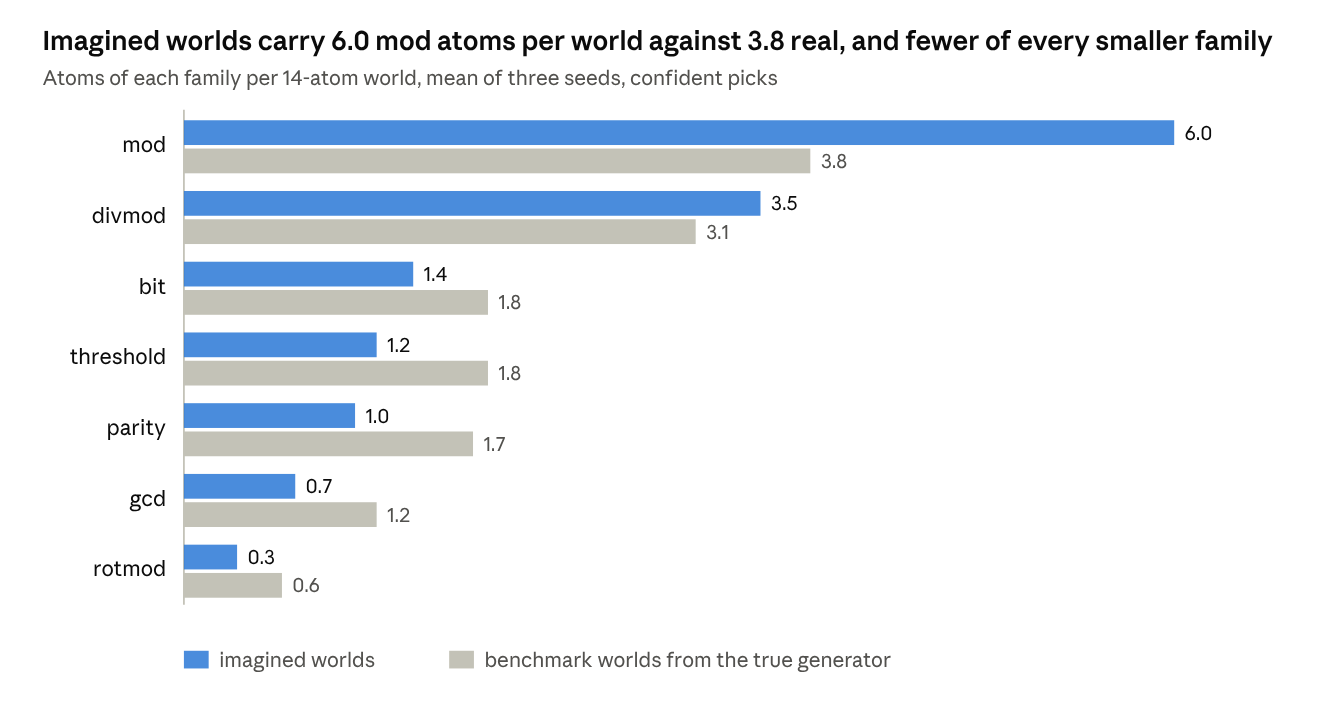
\includegraphics[width=\linewidth]{fig-mix.png}
\caption{Atoms of each family per 14-atom world, imagined worlds against benchmark worlds from the true generator, mean of the three seeds, confident picks.}
\label{fig:mix}
\end{figure}

Figure~\ref{fig:mix} gives the family mix. Imagined worlds carry 6.1, 5.3 and 6.5 mod atoms per world on the three seeds against 3.9, 3.2 and 4.3 in the benchmark, and correspondingly fewer atoms of every smaller family. Because a pooled correlation over 230 atoms is a correlation between a block of 125 to 132 mod atoms and everything else, a shift in how mod worlds are weighted moves it even when every atom's rate is right. The atoms that the self-model binding files as import-only, about 20 of mod and 5 of divmod with true discovery rates below 0.10, are present in benchmark worlds and never in imagined ones, and they lie outside every number above.

\section{Diagnosis of the remaining error}

The family mix is wrong because the model's distribution over group sets is wrong, and it is wrong in one place. At seed 644101 the learned $\pi$ puts a mod group in 64\% of imagined worlds while mod appears in 35\% of the training worlds. The posterior over group sets assigns the true family triple to 50\% of training worlds, and every one of the six most common confusions is a rotmod world. Worlds built from divmod, rotmod and threshold are read as divmod, gcd and threshold in 59 cases, worlds from divmod, mod and rotmod as divmod, mod and parity in 51, and worlds from mod, rotmod and threshold as gcd, mod and threshold in 40. The model has no group set that contains rotmod because it has no rotmod group, so all ten rotmod triples receive no mass and their worlds are spread over the sets that share two families with them. Many of those contain mod.

Rotmod never receives a group at any count from 6 to 9. At 7 groups the fit spends the seventh group on one to three stray atoms, and at 8 and 9 it splits mod, bit or threshold instead. A restart that frees the smallest group for the atoms the model explains worst raises the held-out likelihood at 7 groups from $-11{,}595$ to $-11{,}540$, but it frees the group for two mod atoms. Ranked by how badly the model explains them, the seven grouped rotmod atoms stand 28th to 132nd of 232, and 46th to 154th when the margin is taken per earn. They are not misfits. A rotmod atom filed under mod is explained as well as a true mod atom.

The reason is the import rate $f$. It is a free parameter per atom, fitted to the earns the posterior attributes to worlds where the atom's group is absent. Seven of the ten trained rotmod triples do not contain mod, so most of a rotmod atom's earns fall in worlds the model reads as mod-free, and $f$ rises to absorb them at the same cost the model would pay for a genuinely imported atom. Misfiling is free to the likelihood. The import-only atoms, whose rates are measured at 0.01 to 0.09, say what $f$ should be for any atom that really is being imported. Tying $f$ for grouped atoms to that range would make earns outside the group's worlds costly, and a rotmod atom would then be explained far better by a group of its own. This is the next change, and it was not made before this writing.

Two errors in the sampling of imagined worlds hid this diagnosis for a day. The imagination routine applied the viability filter by redrawing the group set after a rejected world, which shifted mod presence from 0.53 to 0.41 under the six-group model, while the true generator redraws the atoms and leaves presence alone. The raw sampler redrew the group set whenever a drawn world left one of its groups unused, which happens often for a group of one to three atoms, so sets containing a small group were under-sampled and the diagnostics built on it reported mod presence of 0.36 when $\pi$ said 0.64. Both now keep the set and redraw the atoms. With the filter on, a kept world takes 1.6 draws on average and one set in 801 exhausted its 40 attempts.

A divmod gap reported in the first pass, imagined 0.53 against a ceiling of 0.97, was the old benchmark's. Its ceiling over all 50 divmod atoms was carried by a few atoms with discovery rates near zero, and on the atoms the model also imagines the ceiling is 0.49 to 0.71, which the model meets.

\section{Lessons bought with wrong results}

\begin{enumerate}[leftmargin=*]
\item Score a world model against the distribution the agent lived in. A benchmark drawn from a wider pool measured a shift the model could not have learned, and the model was faulted for being right about its own experience.
\item Report fidelity per family against a ceiling computed on the same atoms, with the per-atom error beside it. A pooled correlation over families of very different sizes and spreads is dominated by the largest family's within-family noise. Here it read 0.17 to 0.39 while every family was at its ceiling.
\item A sampler that rejects a draw must redraw the atoms and never the group set. Two routines broke this rule in different ways and both hid the same error. The check that catches it is direct: the sampler's marginal over group sets must equal $\pi$.
\item The agent's confident picks are the evidence to fit on. One consistent hypothesis within budget means a correct pick 90\% of the time against 26\% above sixteen, and fitting on those picks raised group recovery from adjusted Rand 0.45 to 0.67 to 0.90 to 0.93 on two seeds.
\item Check identifiability for the structure to be recovered, not only for the rates. A free nuisance parameter per atom, the import rate, made a wrong group assignment costless, and no amount of restarting or likelihood selection can find a structure the likelihood cannot see.
\item Validate the simulation against the truth before using it inside the model. Self-simulation given the true worlds reached 0.91, inside the first model 0.14 to 0.40, which located the fault in the model and not in the procedure.
\item Separate what the agent is from the conditions it is measured under. Removing evaluation mechanisms from training streams changed the agent's discovery rates by enough to make training statistics the wrong target.
\item On a shared machine, cap the worker pool. Twelve workers died of Windows commit exhaustion with other jobs resident. Eight ran.
\end{enumerate}

\section{Limitations and next steps}

Everything here is development on three opened seeds in one environment. No gate was predeclared and no confirmation seed was opened, so none of it is a confirmed claim in the sense the programme uses. The group count was searched over 6 to 8 only, and the expectation-maximization fit has local optima that four restarts do not always escape, as seed 645101 shows. About 25 real atoms with discovery rates below 0.10 are filed as import-only and so, to the agent, do not exist. Imagined worlds are lived with the agent's current policy, and a change of policy requires the self-simulation to be run again. Whether the model extends to family combinations the agent never trained on is not measured.

The next change is the one Section 8 names. Tie the import rate of every grouped atom to the rate measured on import-only atoms, refit, and check three things in order: that rotmod receives a group, that mod presence in imagined worlds falls from 64\% to near 35\%, and that the pooled correlation rises toward its ceiling of 0.78 while the within-family numbers hold. If it does, the feedback loop of Section 5 becomes usable, with the measured discovery rates fixed and prevalence fitted, and the model can be checked against the rarely found atoms it currently discards.

Only then does deployment follow. The model's own predictions of discovery, which Section 7 shows are accurate per atom, are the natural source for the trust and hedge that the earned grouping lacked when C-earned failed on safety at budgets 256 and 512. That test needs a predeclared gate read across the whole budget range, two replications, the handed-set reference beside the earned model, and a forecast committed before the run.

\section{Reproducibility}

The repository is the RSI project at \texttt{projects/rsi}, master at commit \texttt{661b682}, which contains every script and result file below. Seeds are 643101, 644101 and 645101 with 1,600 training worlds each, 1,280 for fitting and 320 for held-out likelihood. The agent runs at 4,096 scans per task over 100 tasks per world, a world admits at least 130 predicates, the import-only threshold on $r$ is 0.10, each fit uses the spectral start plus four shaken restarts plus one misfit restart, and the group count is chosen from 6, 7 and 8. The benchmark draws 1,600 worlds per seed from the training triple pool with random seed 4343 past the development seed. Self-simulation draws 800 worlds. The \texttt{RSI\_WORKERS} environment variable caps the process pool.

\begin{table}[h]
\centering
\caption{Scripts and result files, with the commits that introduced them.}
\label{tab:files}
\small
\begin{tabular}{p{0.40\linewidth}p{0.35\linewidth}p{0.15\linewidth}}
\toprule
File & Purpose & Commit \\
\midrule
\path{rsi/self_world_model.py} & joint world and self model, EM fit, restarts, group-count selection, samplers & c5e1604, bc125af, 3b1617a, 661b682 \\
\path{mechanism_self_simulation.py} & imagined worlds, self-earning with the agent's tie-break, feedback rounds & 2504952, 73cf897 \\
\path{mechanism_pick_confidence.py} & correctness of a pick by the number of consistent hypotheses found & bc125af \\
\path{mechanism_earn_traced.py} & re-earns every training world with the full trace, cached per seed & bc125af \\
\path{mechanism_world_benchmark_trained.py} & the completeness benchmark from the training triple pool, two halves & 73cf897 \\
\path{mechanism_world_completeness.py} & fit, imagine, score per family against per-family ceilings and family mix & 73cf897, 661b682 \\
\path{mechanism_world_benchmark_check.py} & family mix and ceilings of the new benchmark against the old & 08afe7d \\
\path{mechanism_world_filter_diag.py} & real against imagined worlds before and after the viability filter & 73cf897 \\
\path{mechanism_world_pi_diag.py} & learned group-set frequencies against the training triple frequencies, posterior confusions & 73cf897 \\
\path{mechanism_world_groups_diag.py} & group composition and implied family presence by group count & 73cf897 \\
\path{mechanism_world_misfit_diag.py} & where rotmod atoms rank by how badly the model explains them & 8f30a1f \\
\path{mechanism_world_imagine_diag.py} & acceptance and redraws per group set under the retry filter & 661b682 \\
\path{analysis/mechanism-world-completeness-20261010.json} & the results of Section 7 & 661b682 \\
\path{analysis/mechanism-world-benchmark-trained-20261010.json} & the benchmark of Section 6 & 08afe7d \\
\path{analysis/mechanism-self-world-accuracy-20261005.json}, \path{analysis/mechanism-self-simulation-20261005.json} & the first-pass fits and feedback rounds of Sections 4 and 5 & c5e1604, 2504952 \\
\bottomrule
\end{tabular}
\end{table}

The traced earning caches, \texttt{analysis/mechanism-earn-traced-SEED.json} at 6.6 MB each, are rebuilt by \texttt{mechanism\_earn\_traced.py} in about 25 minutes and are not committed. The project's TODO at \texttt{.claude/TODO.md} carries the dated working notes behind every number here. A living copy of this paper with interactive charts is at \url{https://claude.ai/code/artifact/6664a612-30fc-4059-9fa8-71124f164828}.

\end{document}
